\documentclass{article}
\usepackage[utf8]{inputenc}
\usepackage[T1]{fontenc}
\usepackage{graphicx}
\usepackage{hyperref}
\usepackage{geometry}
\geometry{margin=1in}

\title{SYCOPHANT}
\date{Encyclopaedia Britannica (1771)}

\begin{document}
\maketitle

\section*{Historical source}
\textbf{Entry ID:} \texttt{entry-sycophant-251} \\
\textbf{Volume ID:} 191679021 \\
\textbf{Character Count:} 1341

\subsection*{Extracted Text}
SYCOPHANT, an appellation given by the ancient A-
theman to thole who informed the exporation of figs
contary to bay, and hence it is full field in general for all inforners, parafities, flattreets, chests, \&c.

SYDINHAM (Dr.) Thomas), an excellent English phys-
fusion, was the fan of William Sychham of Wanilor Eagle
in Dorforth, and was born there about the year 1934.
He funded at Magdalach-ball, Oxford, but left the univi-
rly when Oxford was performed for King Charles J. and
went to London; where, becoming acquainted with Dr
Thomas Cox, an entirely physician, and perhaps perfua-
eded him to apply himself for the duty of physics, according-
ly, after the garrifon was delivered up to the parliament,
he rented again in Magdalan ball, entered on the body of medicine, and in 16\% was created backache of his faculty at home.
When you made a fellow of All-Souls college, and corti-
nued direct burial years where, leaving the maturity, he
farled to Wedthming become delicer of his faculty atce-
bridge; grew famous for his practice; and was the chief
physician and London they ran 1660 to 16/20, as which
was done he began to be disliked by the good. He died in
1695. His works are highly effecemed both at home and
abroad. He was famous for his cool regimen in the final-
px y-for giving the bark after the paroxym in agues 1 and for



\section*{Source record}
\begin{itemize}
\item \textbf{Dataset:} \texttt{NationalLibraryOfScotland/encyclopaedia\_britannica\_illustrated}
\item \textbf{Dataset Revision:} \texttt{309f765b1ecc83e0a7f7762e44b4a927a7555443}
\item \textbf{Page ID:} \texttt{britannica:309f765b1ecc83e0a7f7762e44b4a927a7555443:train:251} \\
  \textbf{Filename:} \texttt{page-0251-69952e7c4a0f.jpg} \\
  \textbf{Row Index:} 251 \\
  \textbf{SHA256:} \texttt{69952e7c4a0f4026...}
\end{itemize}

\begin{figure}[h]
\centering
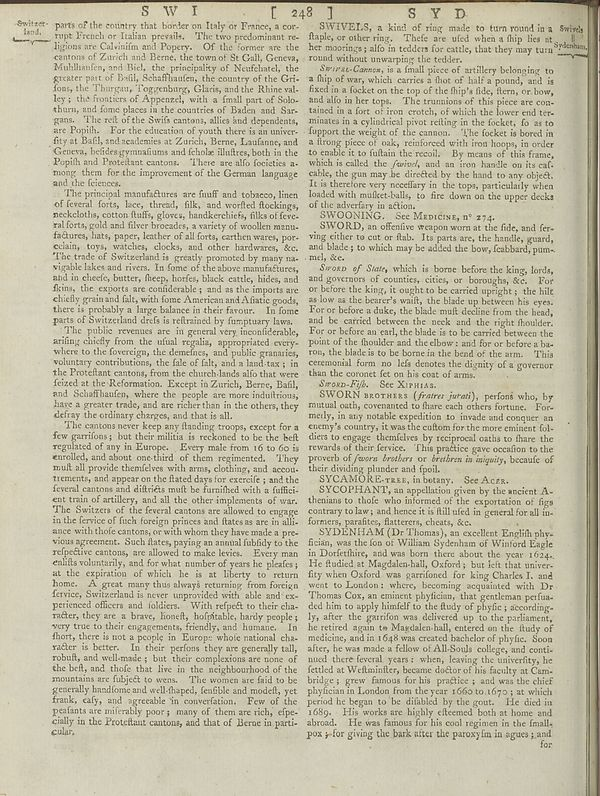
\includegraphics[width=0.85\textwidth]{../scans/page-0251-69952e7c4a0f.jpg}
\caption*{Source scan: \texttt{page-0251-69952e7c4a0f.jpg}}
\end{figure}

\end{document}
